\chapter{Fundamentos da Matemática}
\label{cap:01-fundamentos-da-matemática}

\textbf{Importante:} este capítulo é baseado em \cite{lima2017curso1}.

Estas notas de aula destinam-se aos estudantes da FGV-EMAp que estão cursando a disciplina "Cálculo em uma Variável", com o Prof. Paulo Cezar Pinto Carvalho. Cálculo em uma Variável é a porta de entrada para o mundo da Matemática do ensino superior. Absolutamente todas as áreas da Matemática dependem fortemente das ideias que são desenvolvidas no Cálculo. Mas o que é o Cálculo propriamente? Podemos entender o Cálculo em uma Variável como o estudo das funções reais de uma variável real. Na verdade, a área que faz isso de maneira profunda e formal é a Análise Real, mas o Cálculo pode ser visto como a parte deste estudo que foca na parte operacional. 

Em Cálculo, vocês aprenderão a ``calcular'' (sugestivo, não acham?), enquanto a Análise se preocupa com a formalização das ideias do Cálculo. Mas não nos preocupemos (tanto) com a Análise por agora, no momento certo vocês chegarão a ela. Por agora, o mais importante é aprender as ferramentas que serão utilizadas por vocês pelo resto da vida.

De fato, não são poucas as aplicações do Cálculo. Algumas (dentre milhares) delas são:

\begin{itemize}
	\item Estudo do movimento na Física;
	
	\item Modelos de crescimento populacional;
	
	\item Problemas de maximização e minimização;
	
	\item Funções de distribuição de probabilidade;
	
	\item Modelos epidemiológicos.
\end{itemize}

Através destas notas de aula, eu pretendo ajudar os estudantes a construírem de uma maneira sólida todas as ferramentas que o Cálculo oferece, ilustrando com algumas das suas aplicações. Na prática, estas notas de aula cobrirão mais conteúdo do que o curso cobre (de fato, o tempo é limitado, então nunca dá para cobrir tudo). Nós começaremos bem do começo, dedicando os primeiros capítulos à formação da base teórica necessária ao entendimento do Cálculo (o que se chama de Pré-Cálculo em alguns lugares). Depois nós iremos, progressivamente, apresentar as ferramentas do Cálculo, buscando algum rigor matemático, mas sem transformar estas notas em ``notas de aula de Análise''.

\section{A Linguagem dos Conjuntos}

Antes de falarmos sobre funções, precisamos falar sobre os conjuntos. Na abordagem moderna, ``conjunto'' é uma noção primária. Para nós, no entanto, não interessa um formalismo excessivo sobre conjuntos. Por isso mesmo, nós chamamos esta seção de ``A Linguagem dos Conjuntos'', e não ``Teoria dos Conjuntos''. Assim mesmo, façamos uma definição informal para conjuntos:

\begin{Definition}[Conjunto e elementos]
	Um \textbf{conjunto} é um agrupamento de objetos, que são chamados os seus \textbf{elementos}.
\end{Definition}

Geralmente, nós indicamos um conjunto por uma letra maiúscula. Por exemplo, nós poderíamos definir $A$ como o conjunto formado pelos elementos $1$, $2$, $3$, $4$ e $5$.

Se um conjunto é algo que possui elementos, intuitivamente nós podemos nos perguntar se um certo objeto pertence a um conjunto ou não. Esta é a relação básica entre um objeto e um conjunto, a qual nós definiremos agora.

\begin{Definition}[Pertinência]
	Sejam $A$ um conjunto e $x$ um objeto qualquer. Se $x$ é um dos elementos de $A$, nós dizemos que \textbf{$x$ pertence a $A$} e escrevemos
	
	$$
	x\in A.
	$$
	Por outro lado, se $x$ não é um dos elementos de $A$, nós dizemos que \textbf{$x$ não pertence a $A$}, e escrevemos
	
	$$
	x\notin A.
	$$
\end{Definition}

Vocês poderiam se perguntar agora: ``quais tipos de objetos nós podemos agrupar em conjunto?''. A resposta simples é: qualquer coisa. Números, letras, frutas, cidades, até mesmo conjuntos, etc. podem ser elementos de um conjunto. E, ao mesmo tempo, um conjunto não precisa ter elementos todos de um mesmo tipo. Por exemplo, um conjunto $A$ cujos elementos são: $3$, banana, Brasil e $B$(onde $B$ é um conjunto) é um conjunto perfeitamente válido.

Dado que qualquer coisa pode ser elemento de um conjunto, nós podemos nos perguntar, dado um conjunto, como saber se um elemento pertence ou não a este conjunto. Isso costuma acontecer por meio de uma regra, que permita dizer sobre a pertinência de um certo objeto a um conjunto.

\begin{Definition}[Conjunto bem-definido]
	Diz-se que um conjunto $A$ fica \textbf{bem-definido} quando ele possui uma regra que permita decidir se um objeto $x$ qualquer pertence ou não a $A$.
\end{Definition}

No nosso exemplo anterior, nós temos que $3\in A$, mas $\text{Bulgária}\notin A$. A partir de uma regra que torne um conjunto bem-definido, nós podemos definir notações convenientes para representar os elementos de um conjunto.

Vamos fazer alguns exemplos para apresentar tais notações.

\begin{Example}
	Considere um conjunto $A$ cujos elementos são os números $1$, $2$, $3$ e $4$. Uma forma bem visual de se representar este conjunto é a seguinte:
	
	\begin{center}
		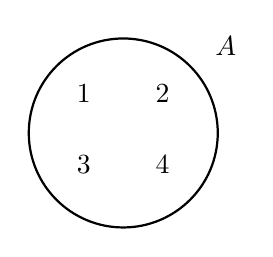
\begin{tikzpicture}
			% Desenha a curva fechada para o conjunto A
			\draw[thick] (0,0) ellipse (1.2cm and 1.2cm);
			
			% Rótulo do conjunto A
			\node at (1.3, 1.1) {$A$};
			
			% Elementos dispostos dentro do conjunto
			\node at (-0.5, 0.5) {$1$};
			\node at (0.5, 0.5) {$2$};
			\node at (-0.5, -0.4) {$3$};
			\node at (0.5, -0.4) {$4$};
		\end{tikzpicture}
	\end{center}
	
	Esta forma visual de representação é chamada de \textbf{Diagrama de Venn}.
\end{Example}

\begin{Example}
	Considere o conjunto $B$ formado pelos elementos $1$, $3$, $5$ e $7$. Uma forma de se representar este conjunto é simplesmente descrevendo os seus elementos, com a seguinte notação:
	
	$$
	B = \{1, 3, 5, 7\}.
	$$
\end{Example}

\begin{Example}
	Considere o conjunto $C$ por todas as potências de $2$). Uma forma de se representar este conjunto é como:
	
	$$
	C = \{\cdots, 1/4, 1/2, 1, 2, 4, 8, \cdots\}.
	$$
	
	Implicitamente, é possível perceber que $C$ possui um padrão, e deduzir quais são todos os infinitos elementos de $C$. Por outro lado, nada nos garante que a regra se mantém para sempre. Uma outra maneira de se definir este conjunto poderia ser a seguinte:
	
	$$
	C = \{n; \text{$n$ é uma potência de $2$}\}.
	$$
\end{Example}

É muito comum, na verdade, esta última forma de representação. De fato, muitas vezes nós lidamos com conjuntos formados por elementos que satisfazem a alguma certa propriedade. Suponhamos, por exemplo, que um certo conjunto $X$ é definido a partir de uma certa propriedade que chamaremos de $P$ (ou seja, todos os elementos de $X$ possuem a propriedade $P$ e, reciprocamente, um elemento só pode pertencer a $X$ se possuir a propriedade $P$). Então, podemos descrever este conjunto como:

$$
X = \{x; \text{$x$ possui a propriedade $P$}\}.
$$

Seria possível também que a propriedade $P$ se referisse a elementos de um certo conjunto fundamental $E$. Por exemplo, tomando $E = \{1, 2, 3, 4, 5, 6, 7, 8\}$, e $P = \text{é um número par}$, poderíamos montar um conjunto $A$ da seguinte forma:

$$
A = \{x\in E; \text{$x$ é um número par}\} = \{2, 4, 6, 8\}.
$$
Repare que $10$ é um número par, mas $10\notin A$, porque $10\notin E$.

Por outro lado, suponha que nós adotamos a seguinte propriedade $Q$: $Q = \text{é um número maior do que 10}$. Neste caso, nenhum elemento de $E$ satisfaz esta propriedade. Se quisermos montar um conjunto definido por:

$$
B = \{x\in E; \text{$x$ é um número maior do que 10}\},
$$
o conjunto $B$ não possuirá nenhum elemento. Neste caso, dizemos que $B$ é um conjunto vazio.

\begin{Definition}[Conjunto vazio]
	Considere um conjunto $\emptyset$ tal que, qualquer que seja $x$, tem-se $x\notin\emptyset$. Este conjunto é chamado o \textbf{conjunto vazio}.
\end{Definition}